\documentclass[12pt]{article}
\usepackage[margin=1in]{geometry}
\usepackage{times}
\usepackage{setspace}
\usepackage{parskip}
\usepackage{amsmath}
\usepackage{booktabs}
\usepackage{graphicx}
\usepackage{float}

\onehalfspacing
\pagestyle{plain}

\begin{document}

\noindent Kidus Bezuayeho \\
May 2026 \\
Fintech Write-Up

\section*{Question 0}

\subsection*{Part (a)}

For an OLS regression to yield a causal estimate, it would need to be true that there is no omitted variable bias, no selection bias, and no reverse causality. This is because omitted variable bias can lead to a false relationship when a third factor drives both variables, selection bias can cause results to reflect the type of stocks that attract herding rather than herding itself, and reverse causality can make buying appear to predict returns when investors are actually reacting to expected returns.

\subsection*{Part (b)}

One confounder is media and news coverage. When a sector gets a lot of media attention, Robinhood users rush to buy stocks in that sector while prices rise across the board, even for companies that are not actually benefiting. When prices eventually fall back down, it looks like the buying caused the drop when really the media hype was responsible all along.

Another confounder is earnings announcements. Before a company reports its earnings, speculation drives increased buying and price run-ups. If the report disappoints, prices fall, making the buying appear to have caused the drop when the earnings miss was the real cause.

\subsection*{Part (c)}

The authors attempt to address identification concerns in several ways. One approach is controlling for lagged returns, which minimizes the effects of stocks naturally bouncing back after a big move. If a stock shoots up one day, it often falls the next simply because of normal price behavior, not because of any buying activity. By controlling for lagged returns, the authors can show that the negative returns they find are not just this normal bounce-back effect.

Another way they attempted to address this concern was with the outage analysis so that they could isolate the specific impact of Robinhood trading itself. On days when Robinhood went down, users who wanted to buy certain stocks simply could not. By comparing trading activity on outage days to normal days, the authors could show that the drop in trading was directly tied to Robinhood users being locked out, not to any other factor, making it much harder to argue that a third variable was driving the results.

\section*{Question 1}

\subsection*{Part (a)}

Please see code, Solutions/Question\_1.py for how I calculated 1a, left comments in the code.
For user change, I had to calculate it with a 3 day gap between days. Since the data set was a randomized subset of the full data, many data points did not have the previous day avaibale. 
I choose the 3 day gap as it would allow me observe Friday to MOnday changes while excluding gaps that were to far to be meaningful.
\subsection*{Part (b)}

\begin{figure}[H]
\centering
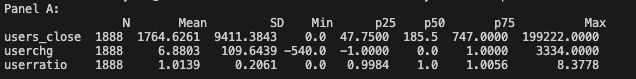
\includegraphics[width=\textwidth]{tables/Panel_A.png}
\end{figure}

\subsection*{Part (c)}

\begin{figure}[H]
\centering
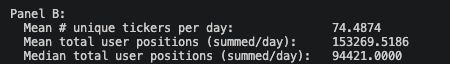
\includegraphics[width=\textwidth]{tables/Panel_B.png}
\end{figure}

\subsection*{Part (d)}

When I compare my summary statistics to the paper, my subsample's distribution is comparable, though the scale differs due to the dataset size. In Panel A, the tendencies in my data are similar to the authors' findings. My median user count of 185.5 and average user ratio of 1.01 mirror the study's median of 160 and mean user ratio of 1.01. Both datasets show a positive skew which confirms that Robinhood user attention is focused on a few stocks. However, the maximums and daily aggregates are smaller in my subsample. The maximum daily user change in my sample is 3,334, compared to 85,193 in the paper. This makes sense because a random sample is less likely to have the massive trading events included. Additionally, my Panel B daily totals are lower. My sample averages 74 unique tickers and 153,000 total positions per day, whereas the full study tracks 7,211 tickers and 15 million daily positions.

\section*{Question 2}

\subsection*{Part (a)}

\begin{figure}[H]
\centering
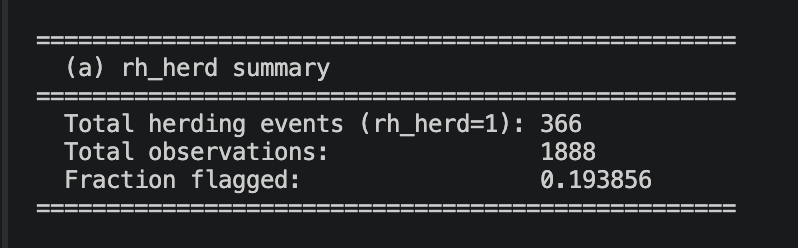
\includegraphics[width=0.75\textwidth]{tables/rh_herd_summary.png}
\end{figure}

\subsection*{Part (b)}

There was a large discrepancy between the number of herding events in my sample and the paper's full dataset. My sample averaged 0.4851 herding events per day while the paper reported 9. I investigated why this difference existed and found it stems from the gaps between observations described in Question 1. The average gap between consecutive observations per ticker was ($\sim$)82 days. Because I cap the lookback at 3 days, most stocks have no valid userratio on any given day, leaving only ($\sim$)2.5 qualifying stocks per day. With such a small pool, 
the top 0.5\% threshold flags roughly 1 out of every 2--3 stocks, making the indicator far less selective than it would be in the full dataset where ($\sim$)74 stocks qualify each day.\\

If I do not use the 3-day gap and instead use the closest prior observation regardless of how long ago it was, the mean and standard deviation of user change become far larger and noisier, no longer comparable to the paper. Therefore, I will stick with the 3-day gap despite it greatly reducing the number of qualifying stocks and herding events per day.

\begin{figure}[H]
\centering
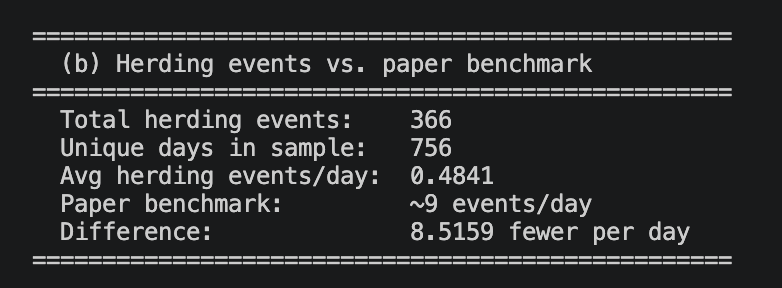
\includegraphics[width=0.75\textwidth]{tables/herding_vs_paper.png}
\end{figure}

\begin{figure}[H]
\centering
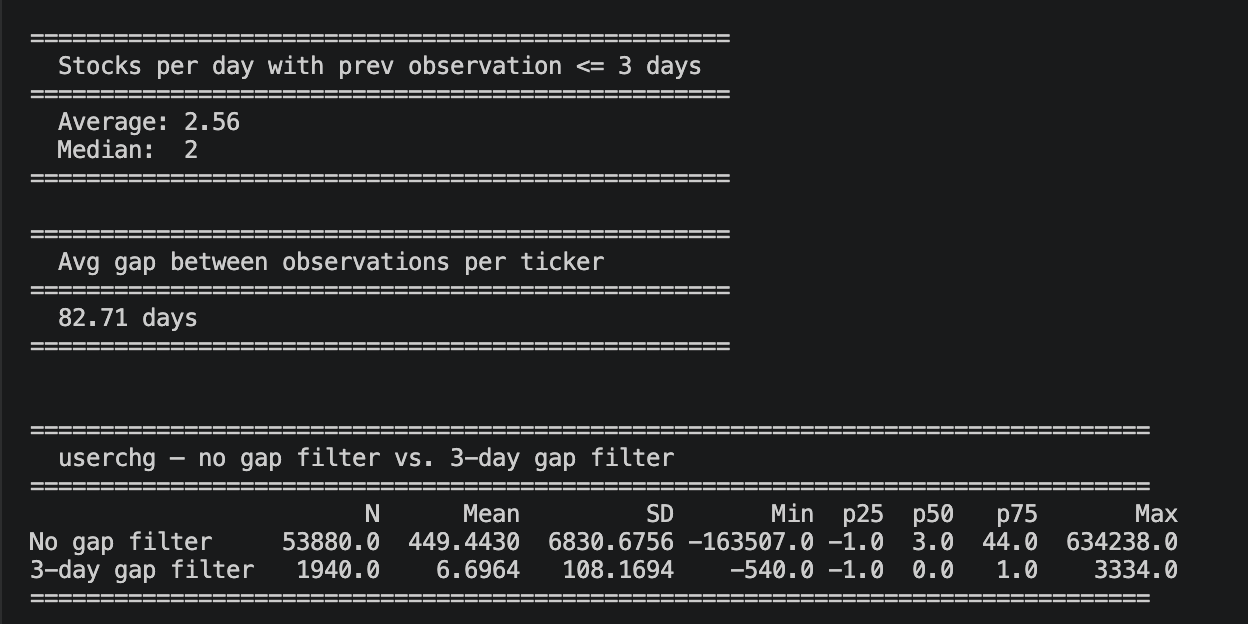
\includegraphics[width=0.75\textwidth]{tables/sparsity.png}
\end{figure}

\subsection*{Part (c)}

There was an issue where results from my sample for returns was lower than teh 366 herding events. I then discoverred that the issue was that many of the stocks seem to be delisted from yfinance.
I included one example where a stock called ACT was mentioned in the dataset (I only included 5 mentions of it) but when I attempted to pull from yfinance you can see it return that it is not returning anything. 
Please see Solutions/debug\_ACT.py to see how I tested this issue.

\begin{figure}[H]
\centering
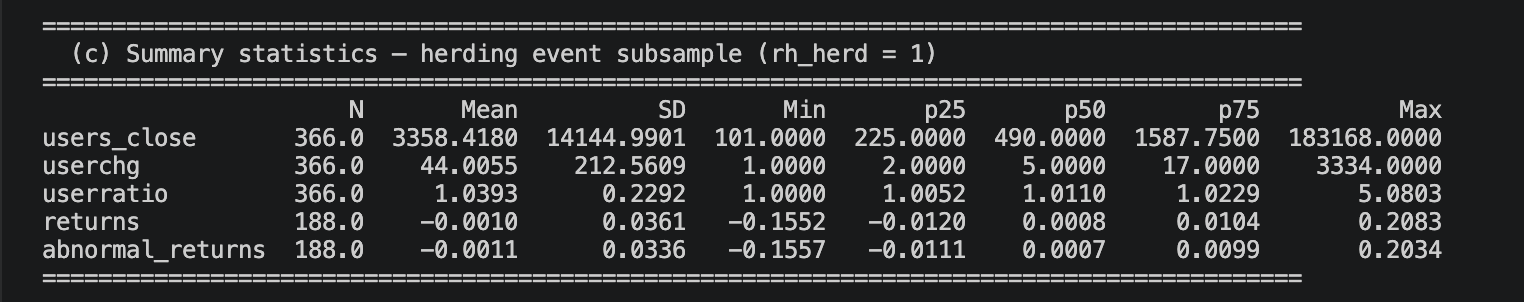
\includegraphics[width=0.75\textwidth]{tables/summary_stats_2c.png}
\end{figure}

\begin{figure}[H]
\centering
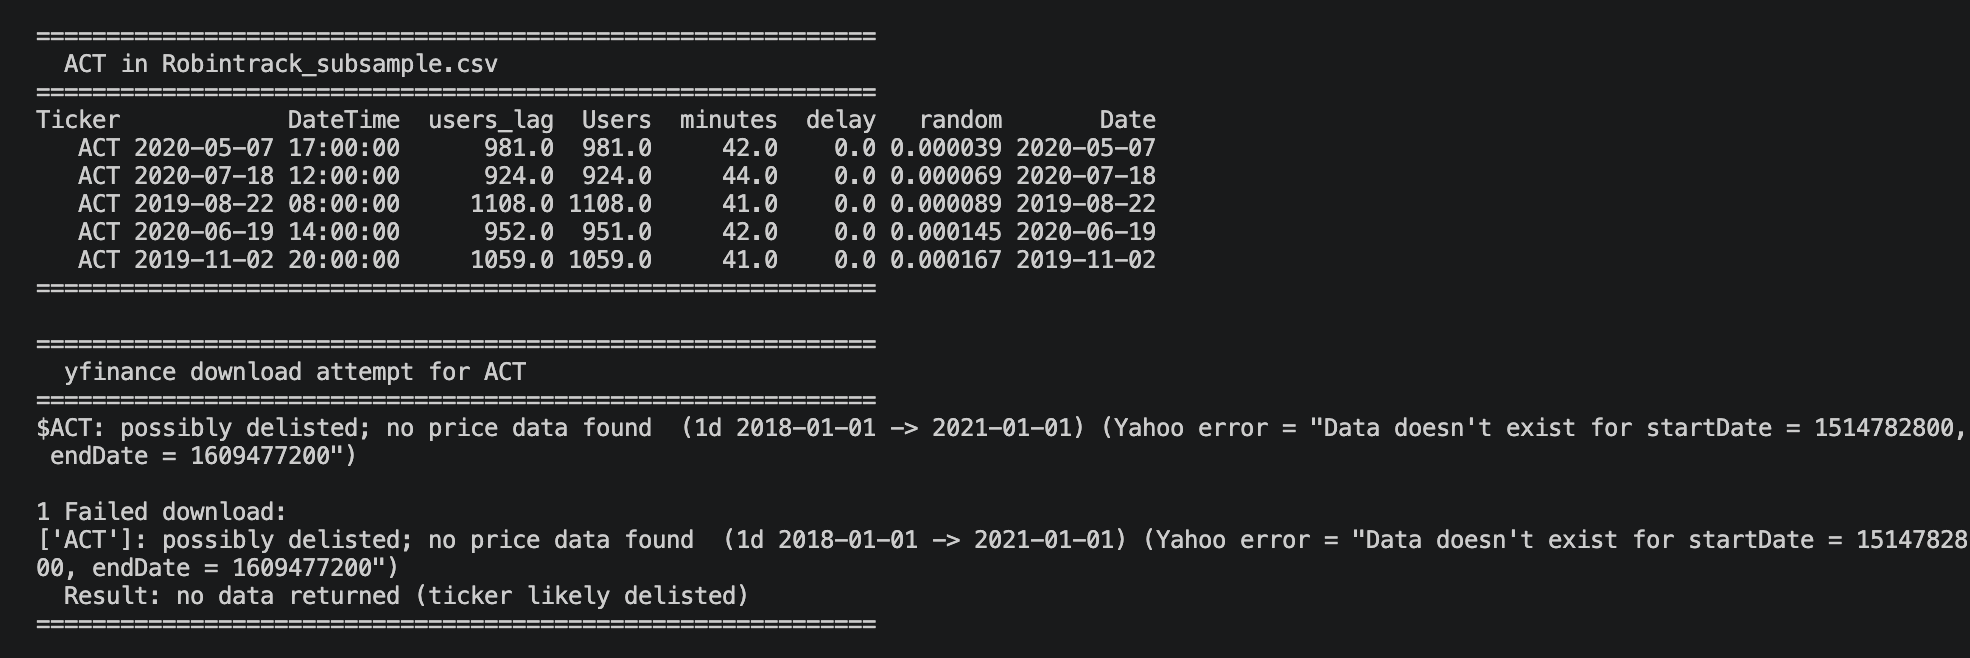
\includegraphics[width=0.75\textwidth]{tables/delisted.png}
\end{figure}

\subsection*{Part (d)}

The graph does show a similar story to the graphs of the study, we can see that after COVID the peaks of the users positions seem to be 
much higher than before COVID. However, due to the my smaller sample size, my graph has much more volaitilty than the paper's graph. This is
most likely why it is not showing the same strong upward trend that the paper's graph.

\begin{figure}[H]
\centering
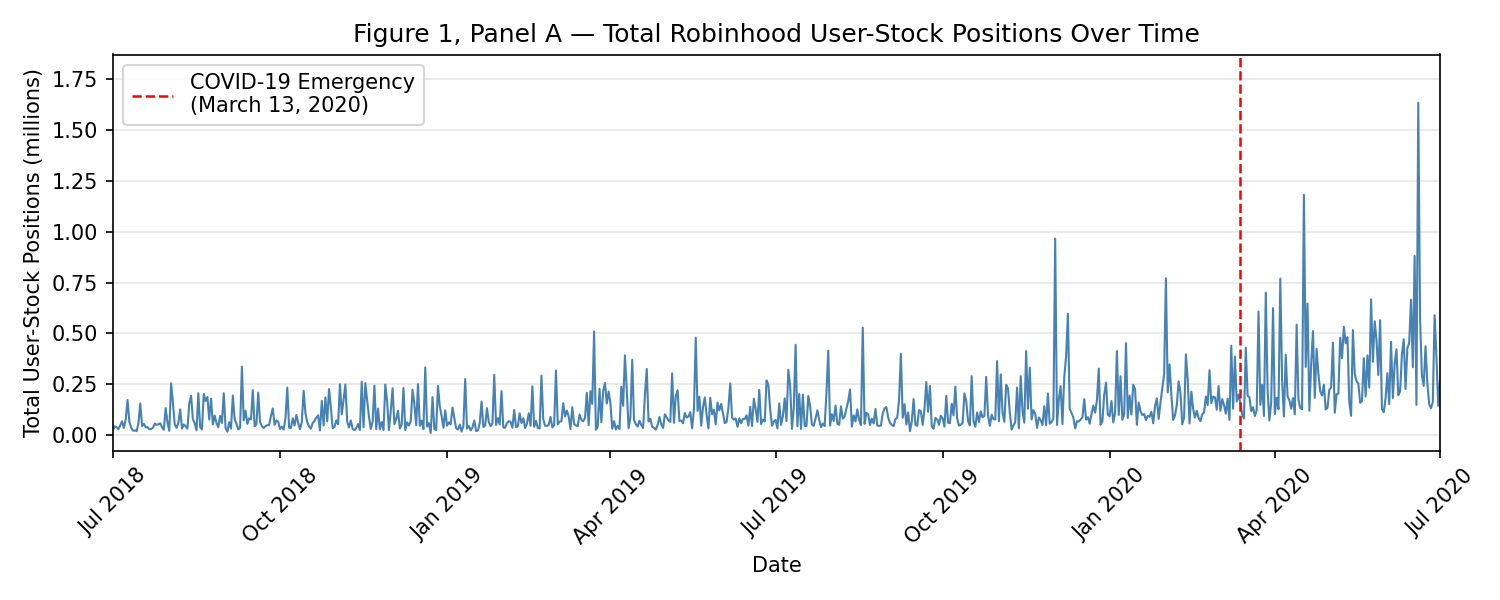
\includegraphics[width=\textwidth]{tables/Total_User_Position_Overtime.png}
\end{figure}

\section*{Question 3}

\subsection*{Part (a)}

For this problem, I calculated user change without the 3-day gap. This is because with the 3-day each day would only have 6 stocks with valid values. 
Since that would just include all 6 for each day, I opted to use the closest prior observation regardless of how long ago it was so that there would be more stocks per day to consider.

\begin{figure}[H]
\centering
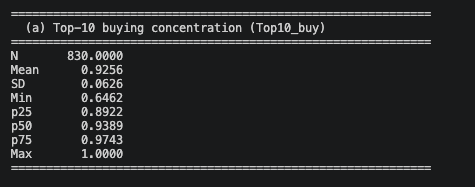
\includegraphics[width=0.75\textwidth]{tables/3a.png}
\end{figure}

\subsection*{Part (b)}

\begin{figure}[H]
\centering
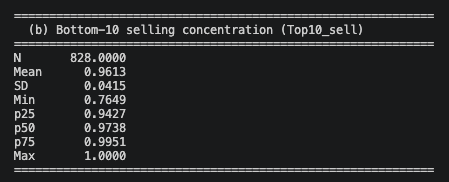
\includegraphics[width=0.75\textwidth]{tables/3b.png}
\end{figure}

\subsection*{Part (c)}

\begin{figure}[H]
\centering
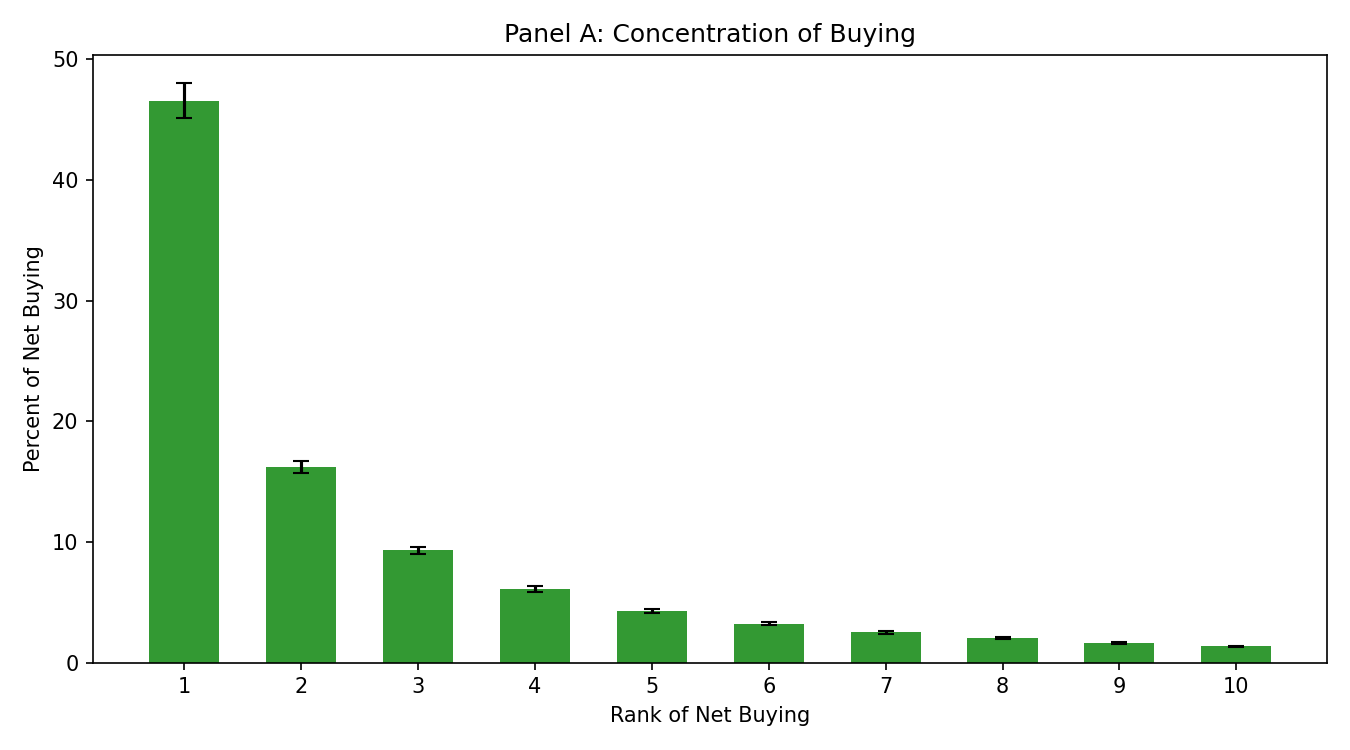
\includegraphics[width=\textwidth]{tables/concentration_buying.png}
\end{figure}

\subsection*{Part (d)}

In this comparison, we can see that the overall shape of the data is identical to that of the study, with rank one having the majority of the concentration, a sharp drop from rank 1 to rank 2, then a slow decline from rank 2 to 10. 
However, the scale of my graph is much larger than that of the paper. My graph shows that the top 10 stocks have a concentration of about 93\% of the buying while the paper's is 35\%. This difference is likely due to my subsample having far fewer stocks observed per day, 
so the top 10 captures nearly all active stocks by construction. Large gaps between observations can also make the increase in users appear more extreme than it really is, which could further inflate concentration in the top 10 stocks.

\end{document}
